%
% simplex.tex
%
% (c) 2025 Prof Dr Andreas Müller, OST Ostschweizer Fachhochschule
%
\documentclass[tikz]{standalone}
\usepackage{times}
\usepackage{amsmath}
\usepackage{txfonts}
\usepackage[utf8]{inputenc}
\usepackage{graphics}
\usetikzlibrary{arrows,intersections,math}
\definecolor{simplexfarbe}{rgb}{0.2,0.6,1.0}
\definecolor{punktfarbe}{rgb}{0.8,0.4,0.6}
\usepackage{ifthen}
\begin{document}

\newboolean{showgrid}
\setboolean{showgrid}{false}
\def\breite{7}
\def\hoehe{4}
\def\h{4}

\begin{tikzpicture}[>=latex,thick]

% Povray Bild
\node at (0,0) {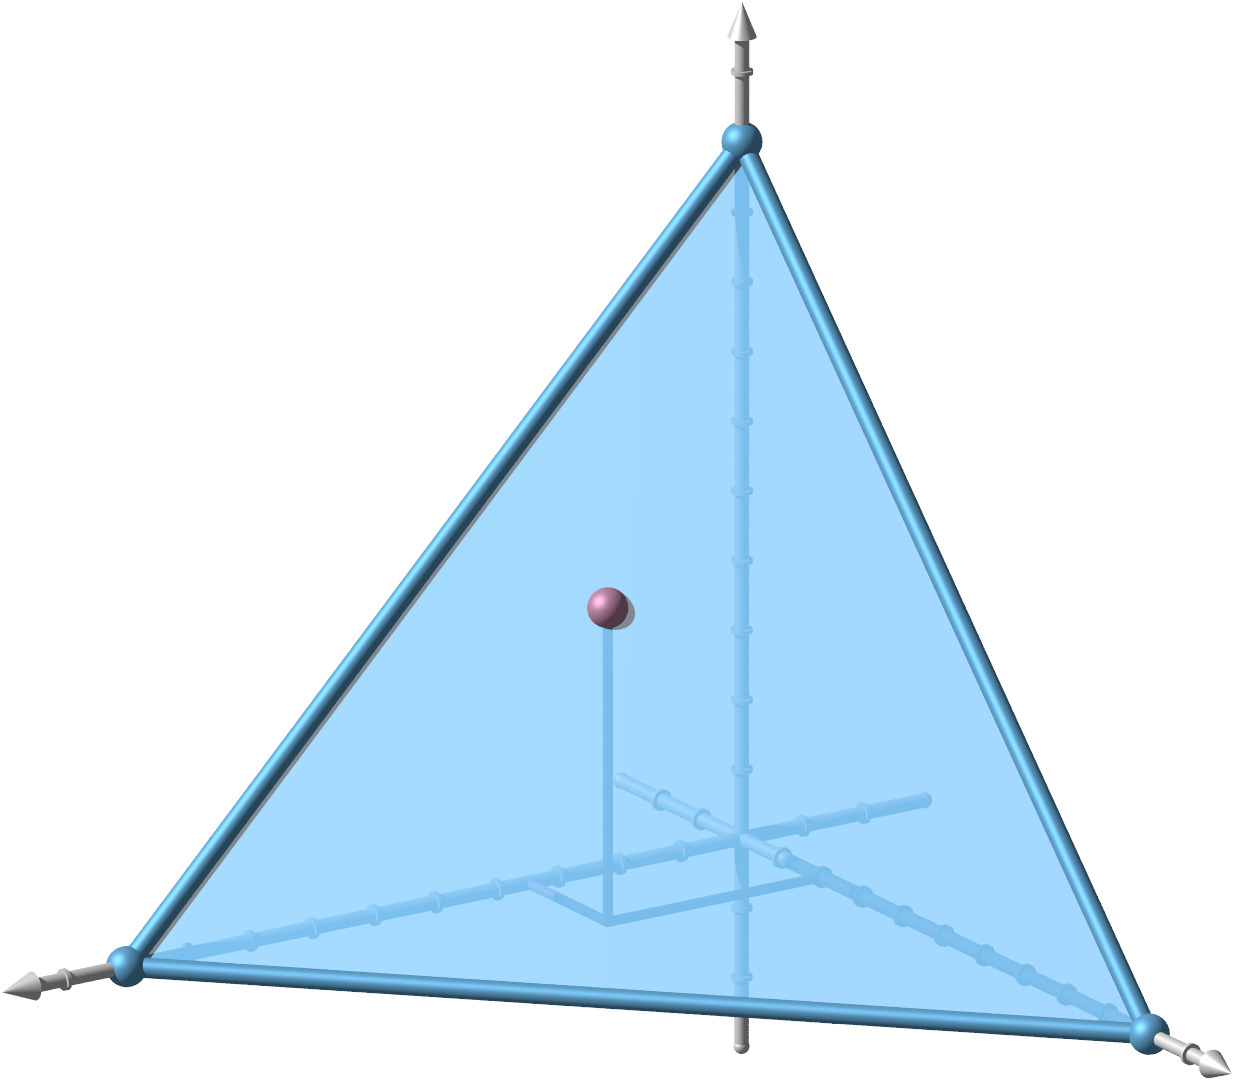
\includegraphics[width=6cm]{2simplex.jpg}};

% Gitter
\ifthenelse{\boolean{showgrid}}{
\draw[step=0.1,line width=0.1pt] (-\breite,-\hoehe) grid (\breite, \hoehe);
\draw[step=0.5,line width=0.4pt] (-\breite,-\hoehe) grid (\breite, \hoehe);
\draw                            (-\breite,-\hoehe) grid (\breite, \hoehe);
\fill (0,0) circle[radius=0.05];
}{}

\node at (-2.9,-1.9) {$t_0$};
\node at (3.0,-2.3) {$t_1$};
\node at (0.4,2.5) {$t_2$};
\node[color=punktfarbe] at (0.25,-0.35) {$P$};
\node at (-2.4,-2.35) {$1$};
\node at (2.6,-2.7) {$1$};
\node at (0.85,1.95) {$1$};
\node[color=simplexfarbe] at (1.2,-0.7) {$\Delta_2$};
\node[color=simplexfarbe] at (0.2,-2.5) {$\Delta_1$};
\node[color=simplexfarbe] at (-1.25,0.0) {$\Delta_1$};
\node[color=simplexfarbe] at (1.95,-0.2) {$\Delta_1$};

\begin{scope}[xshift=-8.5cm,yshift=-2.2cm]
\def\t{0.3}
\draw[color=punktfarbe,line width=0.4pt]
	({\h*\t},0) -- ({\h*\t},{\h*(1-\t)}) -- (0,{\h*(1-\t)});
\draw[color=simplexfarbe,line width=1.4pt] (0,\h) -- (\h,0);
\fill[color=punktfarbe] ({\h*\t},{\h*(1-\t)}) circle[radius=0.07];
\node[color=punktfarbe] at ({\h*\t},{\h*(1-\t)}) [above right] {$P$};
\draw[->] (-0.1,0) -- ({\h+0.5},0) coordinate[label={$t_0$}];
\draw[->] (0,-0.1) -- (0,{\h+0.5}) coordinate[label={right:$t_1$}];
\foreach \x in {0.1,0.2,...,1}{
	\draw ({\h*\x},-0.05) -- ++(0,0.1);
	\draw (-0.05,{\h*\x}) -- ++(0.1,0);
}
\fill[color=simplexfarbe] (\h,0) circle[radius=0.07];
\fill[color=simplexfarbe] (0,\h) circle[radius=0.07];
\node at (0,\h) [left] {$1$};
\node at (\h,0) [below] {$1$};
\node at (0,0) [below left] {$0$};
\node[color=simplexfarbe] at ({0.5*\h},{0.5*\h}) [above right] {$\Delta_1$};
\end{scope}

\end{tikzpicture}

\end{document}

